\chapter{Corpus}
In this study, I use a sample of songs from the Dutch Song Database. The DSD contains metadata of approximately 175,000 songs in the Dutch language, from the Middle Ages up to the twentieth century. It contains love songs, satirical songs, psalms and other religious songs, folksongs, children's songs, St Nicholas songs and Christmas songs, and so on and so forth. For every song the source where the text and/or the melody can be found is indicated. Other metadata that are available for the songs, are (if known) the author, first line, number of stanzas, genre, melody name, stanza form and number of verses. In 2014, the results of the project Dutch Songs On Line, which was a cooperation between the DSD and the Digital Library of Dutch Literature (DBNL), funded with a grant of NWO Medium Investments, became available. In this project, 53,351 full song texts were made accessible online. An additional result of this project are 29,590 songs (a sample of the 53,351 songs) whose lyrics and metadata have all been encoded with TEI compliant XML, which provides publication date, geographical location, melody, classification category and the actual lyrics of a song. This sample is the object of scrutiny of my thesis. The oldest songs in this sample are written in 1260, the most recent songs are from 1991, but the major part of the sample are songs from the seventeenth and the beginning of the eighteenth century (see Figure~\ref{fig:DistSongs}). I have therefore decided to limit the sample to songs that were published between 1550 and 1750, leaving me with a corpus of 22,297 songs.

\begin{figure}[hbt!]
	\centering
	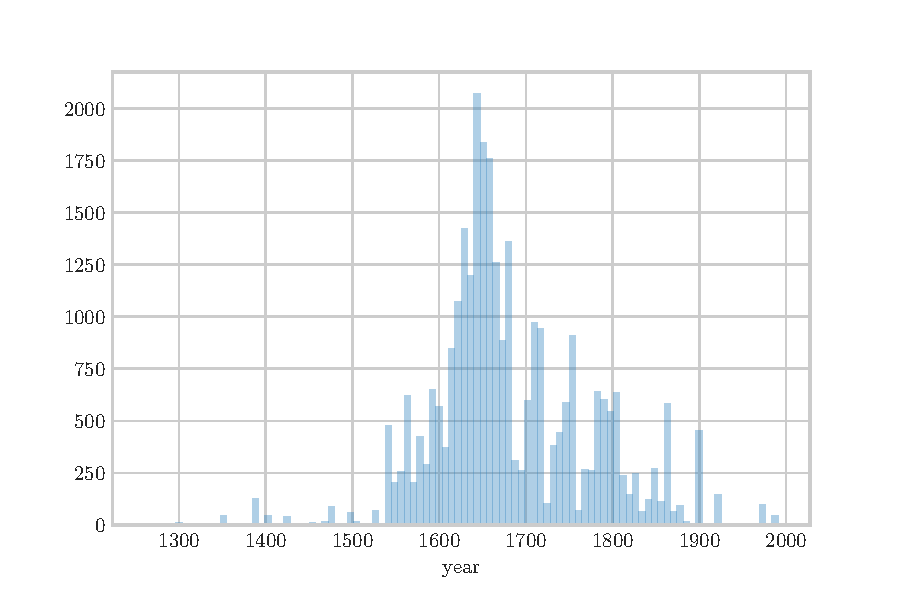
\includegraphics[scale=0.9]{histyeartotal}
	\caption{Distribution of the songs by year (1260-1991) in the sample (\textit{n} = 29,590)}
	\label{fig:DistSongs}
\end{figure}

Since the genre of the song was also tagged in the XML-file, I am able to see how the songs are distributed over the various categories (see Table~\ref{table:SongsCat}). A major part of the songs belong to the genre \enquote{religion}, followed at a distance by \enquote{love and sex},  \enquote{seasons and annual events}, \enquote{formal genres} and \enquote{amusement}. One might ask why a study on topics in song lyrics is useful, since we already have these data on categories, but you can argue with that. This categorical division not only seems a bit arbitrary (when does a song belong to \enquote{work}? What is a \enquote{formal genre}? What are the differences between songs on \enquote{seasons and annual events} and songs on \enquote{occasions}?), there are also more than 9000 songs that have not been assigned to a category. These data thus does not give reliable information about the distribution of songs over different genres. Besides that, the wide-ranging categories don't reveal how subdivisions within a category are distributed. Are all religious songs on the same aspects of religion? Does \enquote{love and sex} mean that some songs are on love, and others on sex? Which words are used to describe the one or the other? In summary, there is an important difference between a genre and a topic, since a genre can comprise many different topics. Topic modeling can give answers to the above questions.

\begin{table}
	\centering
	\begin{tabular}{lr}
		\toprule
		category                  & id        \\
		\midrule
		None                  &  7017 \\
		religion                     &   6914 \\
		love and sex              &   3261 \\
		seasons and annual events &   1033 \\
		formal genres                  &   818 \\
		amusement             &   722 \\
		emotions                &    694 \\
		narratives      &    479 \\
		cycle of life                &    473 \\
		politics and history             &    300 \\
		groups                    &    187 \\
		children                  &    148 \\
		occasions                 &    100 \\
		theatre                   &     90 \\
		work                      &     59 \\
		miscellaneous             &      2 \\
		\bottomrule
	\end{tabular}
	\caption{Number of songs per category (\textit{n} = 22,297)}
	\label{table:SongsCat}
\end{table}

\begin{figure}[hbt!]
	\centering
	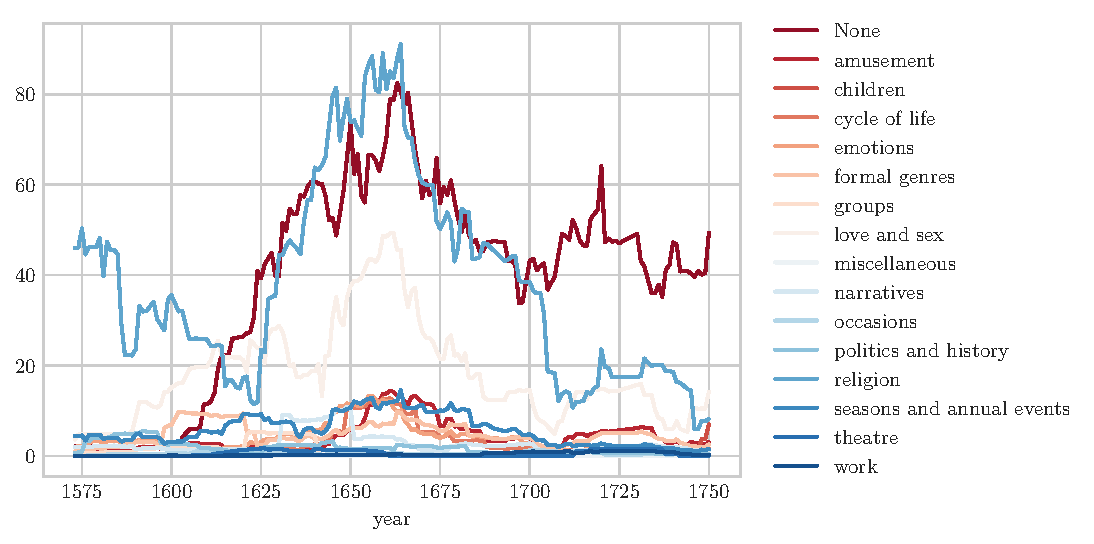
\includegraphics[scale=0.75]{categoriesdist2}
	\caption{Distribution of the categories (\textit{n} = 22,297)}
	\label{fig:CatDist}
\end{figure}

However, the corpus in its current state is not complete yet. It does not include the reprints and appearances of these songs in other songbooks. Since I want to examine which song topics were more prevalent than others, it is necessary to include these data as well. Although the number of lyrics will remain the same, the distribution of the songs can change. Imagine for example that songs on politics and history, which are not very prominent in the corpus based on the data in Table ~\ref{table:SongsCat}, are reprinted so often that their number will increase massively, while songs on love are hardly reprinted. This might influence the distribution of topics. The DSD contains the needed data for this extension of the corpus, but in order to extract them, it is import to understand the terminology that is used in the database. Each first print of a song has a \textit{recordid}, which is the \texttt{id} that is mentioned in the XML-file of a song. A reprint of a song does not contain a \textit{recordid}, but a \textit{herdrukid} instead. Furthermore, each unique song has an \textit{incnormid}. This means that a couple of songs with different \textit{recordid}'s and \textit{herdrukid}'s share the same \textit{incnormid}. I added songs to my corpus with the same \textit{incnormid} and/or \textit{recordid} as the ones already in the corpus, resulting in a corpus of 43,772 songs. Their distribution over time is visualized in Figure~\ref{fig:DistSongsSample}. The next step is to make the lyrics of these songs ready for building topics from it.

\begin{figure}[hbt!]
	\centering
	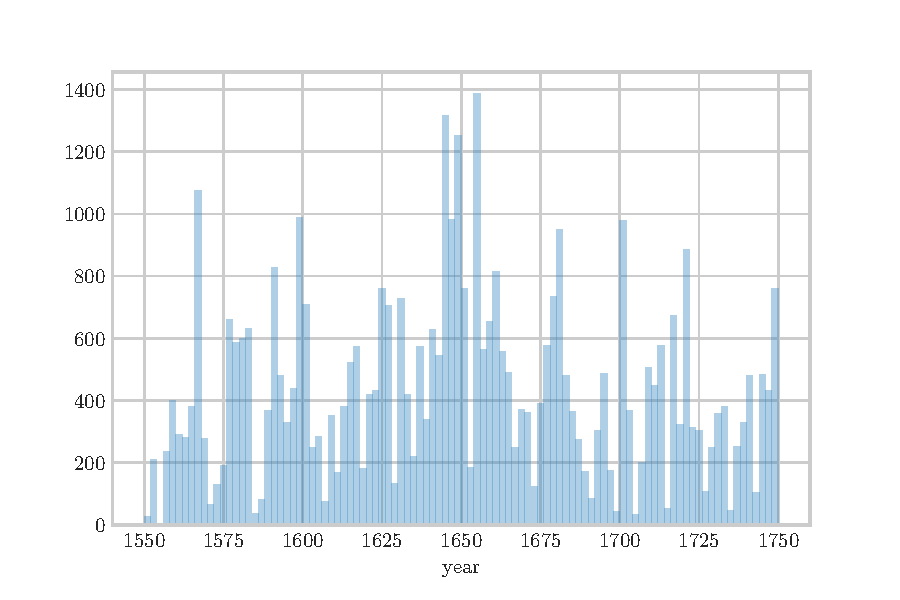
\includegraphics[scale=0.9]{histyearall}
	\caption{Distribution of the songs by year (1550-1750) in the sample (\textit{n} = 43,772)}
	\label{fig:DistSongsSample}
\end{figure}
